


\documentclass[12.5pt, letter, portrait, margin=0mm, innermargin=15mm,
blockverticalspace=10mm, colspace=10mm, subcolspace=8mm]{tikzposter} %Default values for poster format options.








% --------------------------------------------------
% Variables 
% --------------------------------------------------
\newcommand{\ClassName}{EECS 665}
\newcommand{\KUID}{KUID:\@ 2944836}
\newcommand{\Name}{Thomas Atkins}

% Title, Author, Institute
\title{Final Cheatsheet}
\author{Thomas Atkins}
\institute{}

% --------------------------------------------------








\tikzposterlatexaffectionproofoff  %Disables small comment on how the poster was made at bottom of poster




% --------------------------------------------------
% Color Style Definitions
% --------------------------------------------------
% \usepackage[dvipsnames]{xcolor}


\definecolorstyle{newColorStyle}{
    % Define default colors
    % BlueGrayOrange
    \definecolor{colorOne}{gray}{1}
    \definecolor{colorTwo}{RGB}{0, 166, 237}
    \definecolor{colorThree}{RGB}{0, 153, 204}
    \definecolor{white}{RGB}{255,255,255}
    \definecolor{lightGrey}{gray}{0.99}
}{
     % Background Colors
    \colorlet{backgroundcolor}{white}
    \colorlet{framecolor}{colorTwo}
    % Title Colors
    \colorlet{titlefgcolor}{black}
    \colorlet{titlebgcolor}{white}
    % Block Colors
    \colorlet{blocktitlebgcolor}{colorTwo}
    \colorlet{blocktitlefgcolor}{colorOne}
    \colorlet{blockbodybgcolor}{lightGrey}
    \colorlet{blockbodyfgcolor}{black}
    % Innerblock Colors
    \colorlet{innerblocktitlebgcolor}{colorThree}
    \colorlet{innerblocktitlefgcolor}{white}
    \colorlet{innerblockbodybgcolor}{white}
    \colorlet{innerblockbodyfgcolor}{black}
    % Note colors
    \colorlet{notefgcolor}{black}
    \colorlet{notebgcolor}{colorThree!40!white}
    \colorlet{notefrcolor}{colorThree!60!white}
 }

% --------------------------------------------------


% --------------------------------------------------
% Style Definitions
% --------------------------------------------------
\definelayouttheme{newStyle}{
    \usecolorstyle{newColorStyle}
    \usebackgroundstyle{Default}
    \usetitlestyle{Default}
    \useblockstyle{Default}
    \useinnerblockstyle{Default}
    \usenotestyle{Default}
}
% --------------------------------------------------

\usecolorstyle{newColorStyle}
\usetheme{newStyle}




\settitle{ \centering \vbox{
\@titlegraphic \\[\TP@titlegraphictotitledistance] \centering
{ \huge \sc \ClassName{}:} 
\color{titlefgcolor} {\bfseries \Huge \sc \@title}
\hspace{1cm}
{\huge \@author \par} \vspace*{1em} {\LARGE \@institute}

}}









% Commands
\newcommand{\bs}{\textbackslash}   % backslash
\newcommand{\cmd}[1]{{\bf \color{red}#1}}   % highlights command





% --------------------------------------------------
% Color Style Definitions
% --------------------------------------------------
\definecolor{codegreen}{rgb}{0,0.6,0}
\definecolor{codegray}{rgb}{0.5,0.5,0.5}
\definecolor{codepurple}{rgb}{0.58,0,0.82}
\definecolor{backcolour}{rgb}{0.95,0.95,0.92}

\usepackage{listings}
\lstdefinestyle{mystyle}{
    backgroundcolor=\color{backcolour},   
    commentstyle=\color{codegreen},
    keywordstyle=\color{magenta},
    numberstyle=\tiny\color{codegray},
    stringstyle=\color{codepurple},
    basicstyle=\ttfamily\footnotesize,
    breakatwhitespace=false,         
    breaklines=true,                 
    captionpos=b,                    
    keepspaces=true,                 
    numbers=left,                    
    numbersep=5pt,                  
    showspaces=false,                
    showstringspaces=false,
    showtabs=false,                  
    tabsize=2
}
\lstset{style=mystyle}


\usepackage{listings}
% --------------------------------------------------


% -----
% the following writes to an external file called 'foo.hs'
\usepackage{filecontents}
\begin{filecontents*}{foo.py}
import numpy as np

def incmatrix(genl1,genl2):
    m = len(genl1)
    n = len(genl2)
    M = None #to become the incidence matrix
    VT = np.zeros((n*m,1), int)  #dummy variable
    
    #compute the bitwise xor matrix
    M1 = bitxormatrix(genl1)
    M2 = np.triu(bitxormatrix(genl2),1) 

    for i in range(m-1):
        for j in range(i+1, m):
            [r,c] = np.where(M2 == M1[i,j])
            for k in range(len(r)):
                VT[(i)*n + r[k]] = 1;
                VT[(i)*n + c[k]] = 1;
                VT[(j)*n + r[k]] = 1;
                VT[(j)*n + c[k]] = 1;
                
                if M is None:
                    M = np.copy(VT)
                else:
                    M = np.concatenate((M, VT), 1)
                
                VT = np.zeros((n*m,1), int)
    
    return M
\end{filecontents*}
% -----



\begin{document}

\maketitle[ roundedcorners=true,
    titletotopverticalspace=5mm,
    titletoblockverticalspace=5mm]

\begin{columns}%blocks will be placed into columns
    \column{.55}
    \block[]{Minted Test}{
     test
     \lstinputlisting[language=Python]{foo.py}
        this
    }
    \block[roundedcorners=40]{Creating the document}{
        The document begins with:
        \begin{quote}
            \texttt{\bs documentclass[25pt, a0paper, portrait, margin=10mm, innermargin=15mm,
                        blockverticalspace=15mm, colspace=15mm, subcolspace=8mm]\{tikzposter\}\\
                \bs title\{Title\}\\
                \bs author\{Author(s)\}\\
                \bs institute\{Institute \}\\
                \bs titlegraphic\{Logo\}\\
                \bs begin\{document\}\\
                \bs maketitle}
            \\ \dots         \end{quote}

        \begin{tikzfigure}[A figure can be made with \bs \texttt{tikzfigure}; \bs\texttt{figure} does not work]
            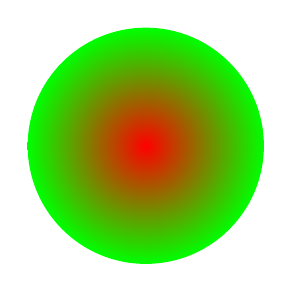
\begin{tikzpicture}
                \draw[draw=none,inner color=red, outer color=green] (0,0) circle (1.5cm);
            \end{tikzpicture}
        \end{tikzfigure}
        \innerblock[]{Inner Blocks}{Inner blocks may be created inside of blocks with the command \bs\texttt{innerblock[{\it options}]\{{\it Heading}\}\{{\it Text}\}} }
        \coloredbox{Text may be highlighted using colored boxes created by \bs\texttt{coloredbox[{\it options}]\{{\it Text\}}}}

    }
    \note[targetoffsetx=-.05\textwidth,targetoffsety=9.5cm,innersep=.4cm,angle=-45,connection]{Optional arguments for the format of the poster}
    \block{The title matter}{
        The title is made by the standard \texttt{\bs ma ketitle[{\it options}]} command where you can alter the \texttt{width}, the spacing between the title and top of the poster (\texttt{titletotopverticalspace}), the bottom of the title to the main content of the poster (\texttt{titletoblockverticalspace}) and the space between the title information and the logo (\texttt{titlegraphictotitleverticalspace}).

        If the default format of the title is not to your liking, you can define the placement of the different items via the \texttt{\bs settitle} command, described in the manual.
    }
    \block{Blocks}{
        Blocks are arranged in a grid, by default, with width by default \texttt{\bs textwdith}.  They are created by the command
        \begin{quote}
            \bs\texttt{block [{\it options}] \{{\it title}\}\{{\it contents}\}}
        \end{quote}
        The title may be left empty, resulting in no title area being created for the block (as seen in a later block to the right).  Further blocks will be placed below automatically, at a distance defined by \texttt{blockverticalspace}.

        If you want to change the position of the title matter or the contents in the block, you may by setting in the options
        \begin{quote}
            \texttt{titleoffsetx, titleoffsety, bodyoffsetx, bodyoffsety}
        \end{quote}
        which let you adjust the vertical or horizontal position of the two parts of the block, respectively.  You can also make, relative to the default width, the title and block body by setting
        \begin{quote}
            \texttt{titlewidthscale, bodywidthscale}
        \end{quote}
        The title's alignment can be set by \texttt{titleleft, titlecenter, titleright}, the body may be shifted vertically by setting \texttt{bodyverticalshift}, and the shape of the block can be altered by setting \texttt{roundedcorners, linewidth}. The inner margins of the title can by set by \texttt{titleinnersep,bodyinnersep}.
    }

    \note[targetoffsetx=24cm, targetoffsety=-9cm,rotate=1,angle=270,radius=8cm,width=.75\textwidth,innersep=.4cm]{
        You can place notes that are ``attached'' to the previous block using the command
        \begin{quote} \texttt{\bs note[{\it options}]\{{\it contents}\}}\end{quote}
        The note is placed by default slightly to the right of a ``target'' in the center of the previous block.  The note style may also allow for a connection between the note and the ``target''.  \\
        The target may be shifted from the default by setting the options  \texttt{targetoffsetx, targetoffsety}, rotated by an angle with \texttt{rotate}, and its width with \texttt{width}.  The placement of the note in relation with the target is given in polar coordinates with \texttt{ radius, angle}. Please observe that notes are always drawn {\bf over} the other objects. They do not affect the placement of blocks.
    }

    \column{.45}


    \begin{subcolumns}
        \subcolumn{.45}
        \block{Subcolumns}{If you want to have an additional subdivision of columns inside a column, you may use the\\ \texttt{\bs subcolumns} environment inside of a column environment.  The functionality is similar to that of columns, but now the widths are relative to the width of the current column.}

        \subcolumn{.5}
        \block{}{An example use of subcolumns is.
            \begin{quote}
                \texttt{\bs begin\{subcolumns\}\\
                    \bs subcolumn\{.6\}\\
                    \bs block\{\dots\}\{\dots\}\\
                    \bs subcolumn\{.4\}\\
                    \bs block\{\dots\}\{\dots\}\\
                    \bs block\{\dots\}\{\dots\}\\
                    \bs end\{subcolumns\}
                }
            \end{quote}
        }
    \end{subcolumns}
    \block[titlewidthscale=.8,bodywidthscale=.9,titleoffsety=9.5mm,bodyoffsety=9mm]{Changing the Poster's Appearance}{
        If the default appearance of the title, background, blocks, and notes is not desired, you may change the colors by calling the color style along with a general layout theme with the commands
        \begin{quote}
            \texttt{\bs usecolorpalette}\{{\em color palette}\}\\
            \texttt{\bs usecolorstyle\{{\em color style}\}}
        \end{quote}
        and
        \begin{quote}
            \texttt{\bs usetheme\{{\em layout style}\}}
        \end{quote}
        where the color palette and style and layout style are either the name of a custom made or one of the offered predefined choices listed in the manual or the comments of this poster's source.  Individual changes can be made to the style of the  background, title matter, blocks, inner blocks, and notes by using one of the following (along with either a custom-designed style or a predefined style listed in the manual or the comments of this poster's source).  These changes are made with the commands
        \begin{quote}
            \texttt{\bs usebackgroundstyle[]\{\}, \bs usetitlestyle[]\{\},\\ \bs useblockstyle[]\{\},\bs innerblockstyle[]\{\}, \bs usenotestyle[]\{\}}
        \end{quote}
        Custom styles for these can be made; this is detailed in the manual.
    }

\end{columns}

\end{document}




\endinput
%%
%% End of file `tikzposter-example.tex'.